\documentclass{beamer}
\usepackage[latin1]{inputenc,colortbl}
\usepackage{epsfig}
\usetheme{Frankfurt}
\setbeamertemplate{navigation symbols}{}
\setbeamertemplate{footline}[page number]
%\newtheorem{definition}{Definition}
\title[Lecture 8: Extensive Form Games with Perfect Information]{Lecture 8: Extensive Form Games with Perfect Information}
\author{INSE 6441/2 DD\\ \vspace{0.2cm} Applied Game Theory and Mechanism Design \\ Fall 2014}
\institute{Department of Computer Science and Software Engineering\\Concordia University}
\date{Novermber 17, 2014}
\begin{document}
%%%%%%%%%%%%%%%%%%%%%%%%%%%%%%%% frame1 title page %%%%%%%%%%%%%%%%%%%%%%%%%%%%%%%%%%%%%%%
%%%%%%%%%%%%%%%%%%%%%%%%%%%%%%%%%%%%%%%%%%%%%%%%%%%%%%%%%%%%%%%%%%%%%%%%%%%%%%
\begin{frame}
\titlepage
\end{frame}
%%%%%%%%%%%%%%%%%%%%%%%%%%%%%%%% frame2 outline page %%%%%%%%%%%%%%%%%%%%%%%%%%%%%%%%%%%%%
%%%%%%%%%%%%%%%%%%%%%%%%%%%%%%%%%%%%%%%%%%%%%%%%%%%%%%%%%%%%%%%%%%%%%%%%%%%%%%

\begin{frame}{Overview}
    \begin{itemize}
     	\itemsep=.5cm
    	\item {\bf Coalition Games}
    	\item Stability and Core
    	\item Fairness and Shapley Value
    	\item Other Solution Conecpts
    \end{itemize}
\end{frame}


%%%%%%%%%%%%%%%%%%%%%%%%%%%%%%%%%%%%%%%%%%%%%%%%%%%%%%%%%%%%%%%%%%%%%%%%%%%%%%
\section{Coalition Games}
\subsection{Cooperative Game Theory}

\begin{frame}{Cooperative Game Theory}
  \begin{itemize}
     \item Cooperative games are a branch of game theory that models cooperation or collaboration between agents.
     \begin{itemize}
        \item Cooperation to perform a set of tasks that requires different expertise.
        \item Agents do not have enough resource on their own to perform the tasks.
        \item Examples:
        \begin{itemize}
            \item Robots have the ability to move objects in a plant, but multiple robots are required to move a heavy box.
            \item Transportation domain: agents are trucks, trains, airplanes, ships... a task is a good to be transported.
        \end{itemize}
    \end{itemize}
    \item \textbf{Issues:}
        \begin{itemize}
            \item Coalition formation.
            \item Rewarding members when a task is completed.
        \end{itemize}
  \end{itemize}
\end{frame}

%%%%%%%%%%%%%%%%%%%%%%%%%%%%%%%% frame14 Background and Literature Review %%%%%%%%%%%%%%%%%%%%%%%%%%%%%%%%%%%%%
%%%%%%%%%%%%%%%%%%%%%%%%%%%%%%%%%%%%%%%%%%%%%%%%%%%%%%%%%%%%%%%%%%%%%%%%%%%%%%
\begin{frame}{Cooperative Game Theory}
    \begin{itemize}
         \item Cooperative games are a branch of game theory that models cooperation or collaboration between agents within coalitions.
    \end{itemize}
    \begin{definition} [Coalition]~\\
       We have a population $N$ of $n$ agents, A coalition $C$ is a set of agents: $C \in 2^N$.
        \begin{itemize}
            \item $N$ is the set of all agents (or players)
            \item $v:2^N \rightarrow R$ is the \emph{valuation function}. For $C \subseteq N$, $v(C)$ is the value obtained by the coalition $C$
        \end{itemize}
    \end{definition}

    \begin{itemize}
        \item \textbf{Problem:} Given a game $(N,v)$, and assuming all agents in $N$ want to cooperate, how to distribute the gain among the agents?
        \item \textbf{Solution:} a payoff distribution $x \in R^n$ that provides a value to individual agents.

        \begin{itemize}
            \item What are the interesting properties that $x$ should satisfy?
            \item How to determine the payoff vector $x$?
        \end{itemize}

    \end{itemize}
\end{frame}
%%%%%%%%%%%%%%%%%%%%%%%%%%%%%%%%%%%%%%%%%%%%%%%%%%%%%%%%%%%%%%%%%%%%%%%%%%%%%%

\begin{frame}{An Example}

    \begin{center}
        $N = \{1,2,3\}$ \\
        $v(\{1\}) = 0, v(\{2\}) = 0, v(\{3\}) = 0$ \\
        $v(\{1,2\}) = 90$ \\
        $v(\{1,3\}) = 80$ \\
        $v(\{2,3\}) = 70$ \\
        $v(\{1,2,3\}) = 105$ \\
    \end{center}

    What should we do?
    \begin{itemize}
        \item form $\{1,2,3\}$ and share equally $(35,35,35)$?
        \item 3 can say to 1 ``let's form $\{1,3\}$ and share (40,0,40)''
        \item 2 can say to 1 ``let's form $\{1,2\}$ and share (45,45,0)''
        \item 3 can say to 2 ``OK, let's form $\{2,3\}$ and share (0,46,24)''
        \item 1 can say to 2 and 3, ``fine! $\{1,2,3\}$ and (33,47,25)''
        \item ...what is a good solution?
    \end{itemize}

\end{frame}

%%%%%%%%%%%%%%%%%%%%%%%%%%%%%%%% frame15 outline page

%%%%%%%%%%%%%%%%%%%%%%%%%%%%%%%%%%%%%%%%%%%%%%%%%%%%%%%%%%%%%%%%%%%%%%%%%%%%%%
\begin{frame}{Transferable and Non Transferable Utility Games}
    \begin{itemize}
        \item \textbf{Games with Transferable Utility (TU games)}
        \begin{itemize}
            \item Utility is worth the same for all agents.
            \item Utility can be {\color{red} compared} or {\color{red} transferred} between agents.
            \item Irrespective of the division of the coalitional payoff.
            \begin{itemize}
                \item In that case members of the coalition enjoy the same total utility.
            \end{itemize}
        \end{itemize}


        \begin{definition} [Valuation or Characteristic Function]\label{dfn:valuationfunction}
            A \emph{valuation function v} associates a real number $v(C)$ to any subset $C \subseteq N$, i.e., $v:2^N \rightarrow R$ \\
            A {\color{blue}\emph{TU game}} is a pair $(N,v)$ where $N$ is a set of agents and where $v$ is a valuation function.
        \end{definition}



        \item \textbf{Games with Non Transferable Utility (NTU games)} \\
            Agents have different preferences over coalitions and rewards. Non-monetary rewards, i.e. item allocation type of problems where items have different values for different players.
    \end{itemize}
\end{frame}

%%%%%%%%%%%%%%%%%%%%%%%%%%%%%%%%%%%%%%%%%%%%%%%%%%%%%%%%%%%%%%%%%%%%%%%%%%%%%%%
\begin{frame}{Some Properties of Valuation Functions}
    $\forall C_1,C_2 \subseteq N | C_1 \bigcap C_2 = \emptyset, i \in N, i \notin C_1$
    \begin{itemize}
        \item {\color{blue} Additive:} $v(C_1 \bigcup C_2) = v(C_1) + v(C_2)$
        \item {\color{blue} Super additive:} $v(C_1 \bigcup C_2) \geq v(C_1) + v(C_2)$ This is satisfied is many applications, or bigger coalitions will not form.
        \item {\color{blue} Weekly super additive:} $v(C_1 \bigcup \{i\}) \geq v(C_1) + v(\{i\})$
        \item {\color{red} Subadditive:} $v(C_1 \bigcup C_2) \leq v(C_1) + v(C_2)$
    \end{itemize}

    $\forall C_1,C_2 \subseteq N$
    \begin{itemize}
        \item {\color{blue} Convex:} $v(C_1 \bigcup C_2) \geq v(C_1) + v(C_2) - v(C_1 \bigcap C_2)$. Convexity has important properties in cooperative game theory solution concepts.
    \end{itemize}
\end{frame}
%%%%%%%%%%%%%%%%%%%%%%%%%%%%%%%%%%%%%%%%%%%%%%%%%%%%%%%%%%%%%%%%%%%%%%%%%%%%%%
\begin{frame}{Solution Properties}
    Let $x \in R^n$ be a solution of the coalition game $(N,v)$
    \begin{itemize}
        \item {\color{blue} Feasible solution:} $\sum_{i \in N} x(i) \leq v(N)$
        \item {\color{blue} Efficiency:} $\sum_{i \in N} x(i) = v(N)$
        \begin{itemize}
            \item the payoff distribution is an allocation of the entire worth of the grand coalition to all agents.
        \end{itemize}
        \item {\color{blue} Individual rationality:} $\forall i \in N, x(i) \geq v(\{i\})$
        \begin{itemize}
            \item player obtains at least its self-value of payoff.
        \end{itemize}
        \item {\color{blue} Group rationality:} $\forall C \subseteq N, \sum_{i \in N} x(i) \geq v(C)$
    \end{itemize}

    \vspace{0.2cm}

    An {\color{blue} imputation} is a payoff distribution $x$ that is efficient and individual rational.

\end{frame}
%%%%%%%%%%%%%%%%%%%%%%%%%%%%%%%%%%%%%%%%%%%%%%%%%%%%%%%%%%%%%%%%%%%%%%%%%%
%%%%%%%%%%%%%%%%%%%%%%%%%%%%%%%%%%%%%%%%%%%%%%%%%%%%%%%%%%%%%%%%%%%%%%%%%%
\section{Stability and Core}
\subsection{Stability and Core}
%%%%%%%%%%%%%%%%%%%%%%%%%%%%%%%%%%%%%%%%%%%%%%%%%%%%%%%%%%%%%%%%%%%%%%%%%%
\begin{frame}{Stability}
    \begin{itemize}
        \item We all want to work together and get $v(N)$, but we all have different views about how to share the fruits of our work. We can use the values of other coalitions as arguments in favor of a distribution.
        \item A condition for a coalition to form:
            {\color{blue}all} agents prefer to be in it. i.e., none of the participants wishes she were in a different coalition or by herself {\color{blue} $\Rightarrow Stability$ }
        \item The {\color{blue} core} is a stability concept for which no agents prefer to deviate to form a different coalition.
    \end{itemize}
\end{frame}

%%%%%%%%%%%%%%%%%%%%%%%%%%%%%%%%%%%%%%%%%%%%%%%%%%%%%%%%%%%%%%%%%%%%%%%%%%%%%%
\begin{frame} {Solution Concepts: Core}
    The core relates to the stability of the grand coalition: \\ No group of agents has any incentive to change coalition.
    \begin{definition}[$Core$ of a Game $(N,v)$]\label{dfn:core}
        Let $(N,v)$ be a cooperative game, and assume they form the coalition $N$. The core of $(N,v)$ is the set:
        \vspace{0.1cm}
        \begin{center}
            $Core(N,v) = \{x \in R^n | x$ is a group rational imputation$\}$
        \end{center}
        Equivalently,
        \vspace{0.1cm}
        \begin{center}
            $Core(N,v) = \{x \in R^n | x(N) \leq v(N) \wedge x(C) \geq v(C), \forall C \subseteq N\}$ \\
        \end{center}
        \small{$x(N) = \sum_{i \in N} x(i)$}
    \end{definition}

    \begin{itemize}
       \item The coalition is stable $\Leftrightarrow$ The core is not empty
    \end{itemize}

\end{frame}
%%%%%%%%%%%%%%%%%%%%%%%%%%%%%%%%%%%%%%%%%%%%%%%%%%%%%%%%%%%%%%%%%%%%%%%%%%%%%%
\begin{frame} {Example: Core}

    \begin{center}
      $N = \{1,2\}$ \\
      $v(\{1\}) = 5, v(\{2\}) = 5$ \\
      $v(\{1,2\}) = 20$ \\
    \end{center}

    $Core(N,n) = \{(x_1,x_2) \in R^2 | x_1 \geq 5, x_2 \geq 5, x_1 + x_2 = 20\}$

    \begin{figure}[htbp]
        \centering
        %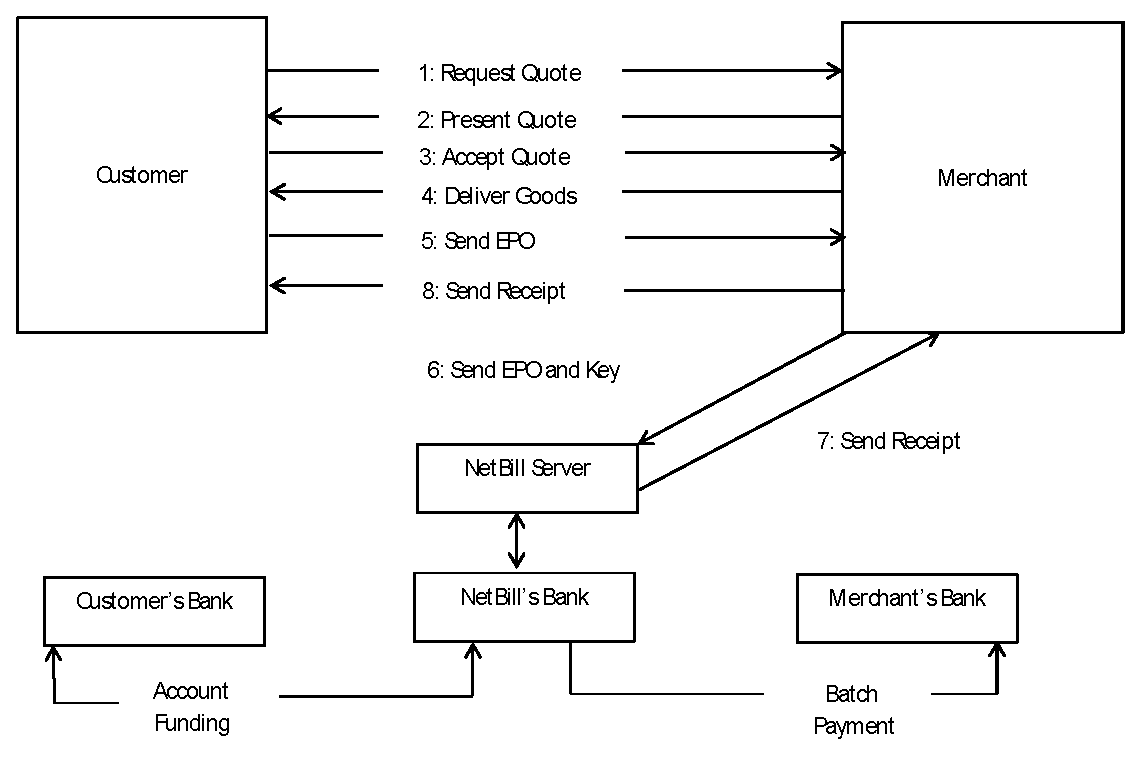
\includegraphics[width=12cm, height=8cm]{figures/figure1.eps}
        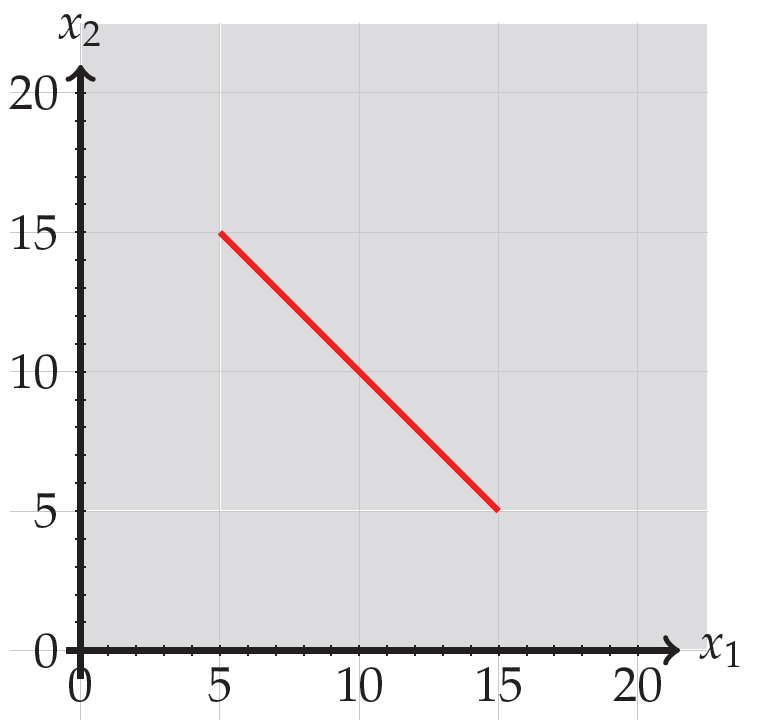
\includegraphics[width=0.3 \columnwidth]{figures/coreex1.png}
        %%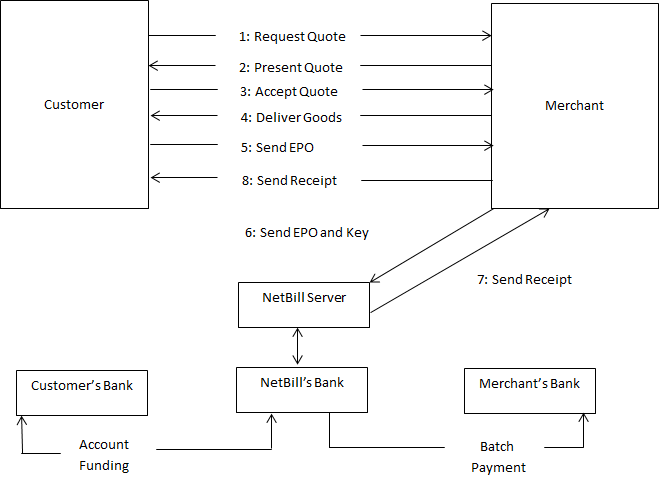
\includegraphics[scale=0.5]{figure1}
        %\caption{The NetBill payment protocol} \label{figure7}
    \end{figure}

    The core may not be fair: the core only considers stability.

\end{frame}
%%%%%%%%%%%%%%%%%%%%%%%%%%%%%%%%%%%%%%%%%%%%%%%%%%%%%%%%%%%%%%%%%%%%%%%%%%%%%
%%%%%%%%%%%%%%%%%%%%%%%%%%%%%%%%%%%%%%%%%%%%%%%%%%%%%%%%%%%%%%%%%%%%%%%%%%%%%
\section{Fairness and Shapley Value}
\subsection{Fairness and Shapley Value}
%%%%%%%%%%%%%%%%%%%%%%%%%%%%%%%%%%%%%%%%%%%%%%%%%%%%%%%%%%%%%%%%%%%%%%%%%%%%%
\begin{frame}{Solution Concepts: Shapley Value}
    \begin{definition} [Marginal Contribution]\label{dfn:marginalcontribution}
        The {\color{blue}marginal contribution} of agent $i$ for a coalition $C \subseteq N \backslash \{i\}$ is $mc_i(C) = v(C \cup \{i\}) - v(C)$
    \end{definition}

    \begin{itemize}
        \item By considering average marginal contribution over all possible subsets of coalitions, we can achieve a fair distribution.\\
        \item Let $\prod(N)$ denote the set of all permutations of the sequence $(1,...n)$. Therefore: $\phi_i(N,v) = \frac{\sum_{\sigma \in \phi_i(N)}}{mc(\sigma)}$
    \end{itemize}

    \begin{definition} [Shapley Value]\label{dfn:shapleyvalue}
        Given a coalitional game $(N,v)$, the Shapley value of player $i$ is given by: \\
        $\phi_i(N,v) = \sum_{S \subseteq N \backslash \left\{i\right\} } \frac{|S|! (|N|-|S|-1)!}{|N|!} (v(S \cup \left\{i\right\}) - v(S))$
    \end{definition}
\end{frame}
%%%%%%%%%%%%%%%%%%%%%%%%%%%%%%%%%%%%%%%%%%%%%%%%%%%%%%%%%%%%%%%%%%%%%%%%%%%%%%%
\begin{frame}{Some Properties}
    \begin{itemize}
        \item The core may not always be non-empty.
        \item Shapley value always exists and is unique.
        \item When the valuation function is {\color{blue}superadditive}, the Shapley value is {\color{blue}individually rational}, i.e., it is an imputation.
        \item When the valuation function is {\color{blue}convex}, the Shapley value is also group rational, hence, it is in the {\color{blue}core}.
        \item A convex game has a non-empty core.
        \item Core and Shapley value are combinatorial problems.
        \item There are other well-known solution concepts: Bargaining set, nucleolus and kernel.
    \end{itemize}
\end{frame}

%%%%%%%%%%%%%%%%%%%%%%%%%%%%%%%%%%%%%%%%%%%%%%%%%%%%%%%%%%%%%%%%%%%%%%%%%%%%%
%%%%%%%%%%%%%%%%%%%%%%%%%%%%%%%%%%%%%%%%%%%%%%%%%%%%%%%%%%%%%%%%%%%%%%%%%%%%%
\section{Other Solution Concepts}
\subsection{Other Solution Concepts}
%%%%%%%%%%%%%%%%%%%%%%%%%%%%%%%%%%%%%%%%%%%%%%%%%%%%%%%%%%%%%%%%%%%%%%%%%%%%%
\begin{frame}{$\epsilon$-Core}
    \begin{itemize}
        \item The core may not always be non-empty, core is a strong condition.
        \item $\epsilon$-core relaxes the core condition.
        \item $\forall S \subseteq N, \sum_{x_i \in S} x_i \geq v(S) - \epsilon$
        \item relative $\epsilon$-Core: $\forall S \subseteq N, \sum_{x_i \in S} x_i \geq (1-\epsilon).v(S)$
    \end{itemize}
\end{frame}

%%%%%%%%%%%%%%%%%%%%%%%%%%%%%%%%%%%%%%%%%%%%%%%%%%%%%%%%%%%%%%%%%%%%%%%%%%%%%
\begin{frame}{$\epsilon$-Core}
    \begin{itemize}
        \item The core may not always be non-empty, core is a strong condition.
        \item $\epsilon$-core relaxes the core condition.
        \item $\forall S \subseteq N, \sum_{x_i \in S} x_i \geq v(S) - \epsilon$
        \item relative $\epsilon$-Core: $\forall S \subseteq N, \sum_{x_i \in S} x_i \geq (1-\epsilon).v(S)$
    \end{itemize}
\end{frame}

%%%%%%%%%%%%%%%%%%%%%%%%%%%%%%%%%%%%%%%%%%%%%%%%%%%%%%%%%%%%%%%%%%%%%%%%%%%%%
\begin{frame}{Kernel}
    \begin{itemize}
        \item Todo
        \item Todo
        \item Todo
        \item Todo
    \end{itemize}
\end{frame}

%%%%%%%%%%%%%%%%%%%%%%%%%%%%%%%%%%%%%%%%%%%%%%%%%%%%%%%%%%%%%%%%%%%%%%%%%%%%%
\begin{frame}{Nucleolus}
    \begin{itemize}
        \item Todo
        \item Todo
        \item Todo
        \item Todo
    \end{itemize}
\end{frame}


\end{document}
